\documentclass{article}
\usepackage{hyperref}
\usepackage[utf8]{inputenc}
\usepackage[english,polish]{babel}
\usepackage{polski}
\usepackage{graphicx}
\graphicspath{ {./} }

\title{Office Space Manager}
\author{Dokument specyfikacji}
\date{8 Listopad 2021}

\begin{document}

\maketitle

\section{Lista członków projektu}
\begin{enumerate}
  \item Grzegorz Nieużyła
  \item Dawid Karolewski
\end{enumerate}


\section{Zakres projektu}

\subsection{Lista cech}
\begin{itemize}
  \item Możliwość rezerwacji, modyfikacji oraz usunięcia rezerwacji miejsca do pracy w wybranym slocie czasowym
  \item Inteligenty wybór bliskiego pomieszczenia w zależności od dokonanych rezerwacji przez ludzi w danym zespole
  \item Powiadomienia mailowe o stanie rezerwacji
  \item Zapis do pliku istotnych informacji o rezerwacji, bądź raportu z nich danego dnia
  \item Gromadzenie statystyk z zarządzania powierzchnia biurową
  \item Dodawanie komentarzy do danej rezerwacji w celu dyskusji pewnych szczegółów związanych z miejscem
  \item Możliwość deklaracji dodatkowego wyposażenia na rezerwowanym stanowisku/pomieszczeniu
\end{itemize}

\subsection{Lista celów produktu}
\begin{itemize}
  \item Brak konieczności zatrudniania osób do zarządzania powierzchnią biurową 
  \item Redukcja kolizji rezerwowanych pomieszczeń
  \item Powiadomienia użytkowników o stanie rezerwacji
  \item Gromadzenie statystyk do dalszych analiz
\end{itemize}

\subsection{Lista produktów}
\begin{itemize}
  \item Aplikacja zarządzająca powierzchnią biurową
  \item Panel administracyjny aplikacji
  \item Dokumentacja 
  \item Szkolenia z użytkowania i administracji systemu
\end{itemize}

\subsection{Harmonogram realizacji projektu}
Realizacja projektu zakłada dostarczenie poszczególnych części w danych ramach czasowych:
\begin{itemize}
  \item 01.11 - Dokumentu wizyjnego
  \item 08.11 - Dokumentu specyfikacji
  \item 15.11 - Proof of concept aplikacji
  \item 22.11 - Dokumentacja systemu
  \item 6.12 - Komponent logowania
  \item 20.12 - Rozwój komponentu rezerwacji
  \item 3.01 - Panel administracyjny
  \item 10.01 - Komponenty notyfikujący oraz raportujący
  \item 17.01 - Testy jednostkowe i manualne aplikacji
  \item 23.01 - Finalnej końcowej wersji implementacji systemu
\end{itemize}

\hspace*{-3cm}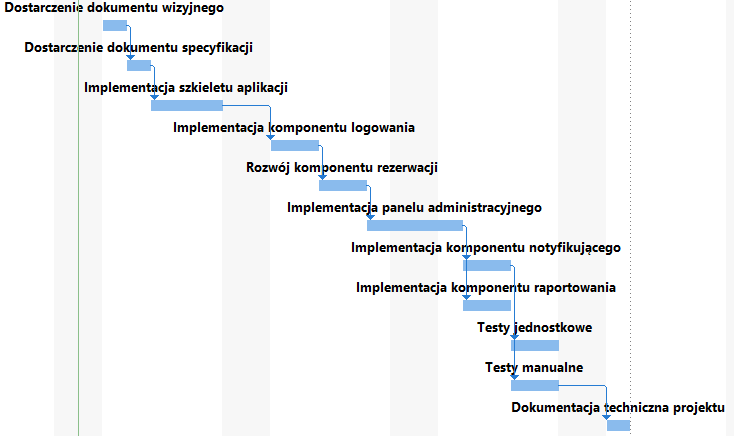
\includegraphics[scale=0.8]{gant}
\begin{center}\textbf{Rys.1} Diagram Gantta \end{center}

\subsection{Opis kosztów projektu}
Koszty, które trzeba ponieść:
\begin{itemize}
  \item Koszty czasu programistów - 80h * 100zł/h = 8000zł
  \item Media (prąd) - 20zł
  \item Zużycie komputera - 100zł
  \item Licencja oprogramowania (Intellij IDEA) - 2000zł * 2 = 4000zł
  \item Koszty serwerów - 2000zł rocznie
\end{itemize}
Koszty, które udało się zredukować to:
\begin{itemize}
  \item Użyte API oraz frameworki są darmowe
\end{itemize}


\section{Przypadki użycia}

Przypadki użycia systemu prezentuje \textbf{Rys.2}. Występuje w nim dwóch głównych aktorów. Użytkownik ma do dyspozycji 3 główne funkcjonalności: zarządzanie rezerwacjami, otrzymywanie powiadomień mailowych oraz dodawanie komentarzy do rezerwacji w aplikacji. Funkcjonalność rezerwacji składa się z 3 podstawowych składowych: rezerwacji, anulacji oraz jej zmiany. Podczas składania rezerwacji użytkownik może zgłosić konieczność użycia dodatkowego sprzętu. Rezerwacja większych pomieszczeń może też być zostać dokonana w sposób inteligentny/automatyczny na podstawie miejsc rezerwacji osób z danego zespołu.

\hspace*{-4cm}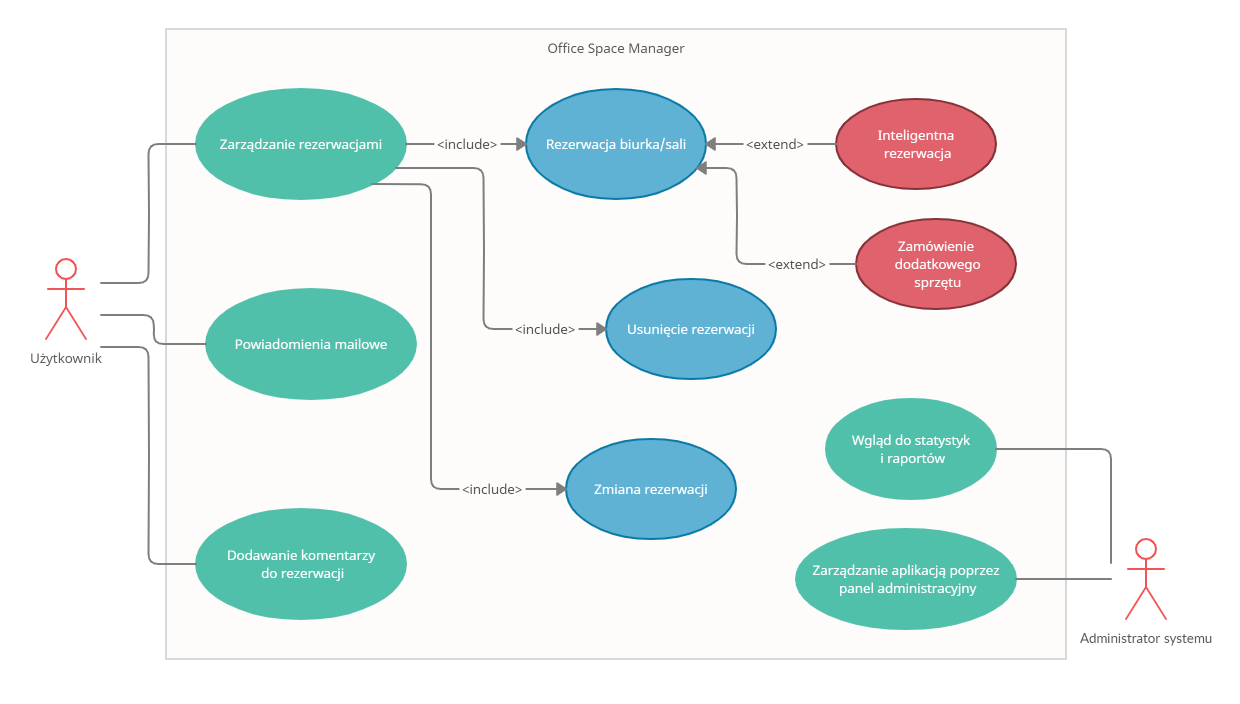
\includegraphics[scale=0.6]{uml}
\begin{center}\textbf{Rys.2} Diagram UML Use Case \end{center}

 Drugim aktorem jest administrator, który za pomocą panelu administracyjnego może zarządzać aplikacją. Ma on też wgląd do statystyk i wygenerowanych raportów systemowych.

\section{Architektura}

Architektura systemu została przedstawiona na \textbf{Rys.3}. Dowolne urządzenie może otworzyć przeglądarkę internetową i po zalogowaniu korzystać z aplikacji.

\hspace*{-3cm}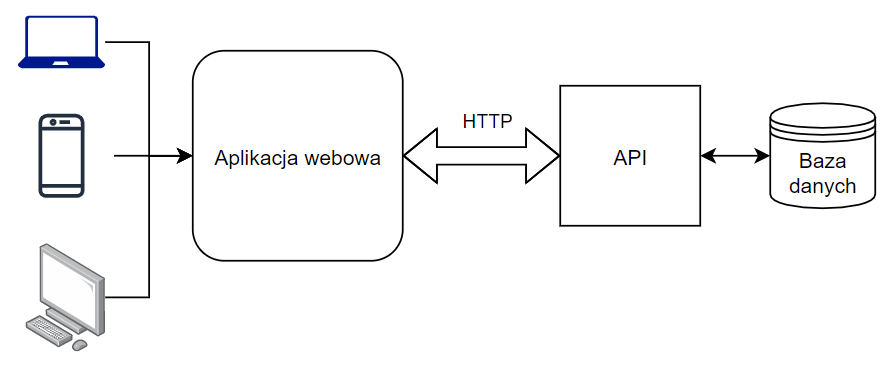
\includegraphics[scale=0.8]{architecture}
\begin{center}\textbf{Rys.3} Architektura systemu \end{center}

Użytkownik poprzez frontend (przyciski, formularze itp.) aplikacji w przeglądarce wyzwala akcje, które poprzez ruch HTTP powodują wysłanie żądań do backendu aplikacji (API). Następnie API przetwarza żądanie często manipulując przy tym bazą danych i po przygotowaniu odpowiedzi wysyła ją z powrotem, która jest wyświetlana użytkownikowi w odpowiedni sposób przez UI aplikacji webowej.


\section{Ryzyko i plan awaryjny}

\begin{itemize}
  \item Kradzież kodu źródłowego
  \item Zmiana wymagań podczas trwania implementacji
  \item Pojawienie się konkurencyjnych rozwiązań
  \item Zwolnienia lekarskie programistów
  \item Awarie sprzętowe - serwer hostujący przestaje działać
  \item Ryzyko powstania luk w bezpieczeństwie systemu
  \item Wyciek wrażliwych danych użytkowników z bazy danych
  \item Nie ukończenie projektu w ustalonych ramach czasowych
\end{itemize}

W celu zabezpieczenia się przed w/w ryzykami przyjęto następujące, które stanowią plan awaryjny:
\begin{itemize}
  \item Zabezpieczenie repozytorium oraz nadawanie praw dostępu tylko developerom
  \item Obniżenie cen systemu oraz wprowadzenie nowych obiecujących feature'ów, które przyciągną klientów
  \item Wydłużenie czasu pracy drugiego developera
  \item Rozważenie hostingu na przynajmniej dwóch serwerach hostujących, aby w przypadku awarii jednego przekierować ruch sieciowy na drugi serwer
  \item Przeprowadzenie dodatkowych skanów bezpieczeństwa przez zewnętrzne serwisy np. Veracode
  \item Rezygnacja z mniej istotnych funkcjonalności w celu ukończenia projektu w założonych ramach czasowych
\end{itemize}


\section{Opis konfiguracji i planu zarządzania produkcją oraz testowaniem}

\subsection{Wymagania systemowe aplikacji i konfiguracja}
W związku z tym, że projektowany system to aplikacja webowa, wyklucza to konieczność stosowania konkretnego systemu operacyjnego. Jedynym wymaganiem koniecznym do używania aplikacji jest stabilne połączenie internetowe oraz zainstalowana dowolna przeglądarka internetowa.

\subsection{Testowanie i kontrola wersji}
System będzie testowany manualnie na maszynie spełniającej wymagania
aplikacji zawarte w poprzednim sekcji oraz przez testy jednostkowe. W przypadku dalszego rozwoju aplikacji, jeśli wystąpi konieczność komunikacji z innymi serwisami, dodane zostaną również testy integracyjne.Kod źródłowy aplikacji będzie przechowywany w serwisie GitHub, w prywatnym repozytorium zarządzany przez system Git.


\end{document}
